\documentclass[a4paper]{article}
\usepackage{array}  
\usepackage{graphicx}
\graphicspath{ {./images/} }
\usepackage[table]{xcolor}% http://ctan.org/pkg/xcolor
\usepackage{geometry}
\geometry{margin=1.25in}
\usepackage{hhline}
\usepackage{environ}
\usepackage{longtable}
 %\geometry{
 %a4paper,z
 %total={170mm,257mm},
 %left=40mm,
 %right=40mm
 %}
 \newcommand{\colWidth}{141mm}

\begin{document} 
\section*{Demo day: \textit{(Demo 2)} Group \textit{(11 - FE.ED)}}

% ------------GOALS----------

\begin{center}
\begin{tabular}{|p{\colWidth}|}
	\hline
	\cellcolor{blue!25}\large
	\textbf{What were your goals?}
	\\ \hline
	\vtop to 180mm{
After our previous demo, we wanted to make our robot more distinctive from the pet food dispensers already available. As a result, we decided to tweak our milestones, bringing in live streaming earlier than we had originally planned in our project plan.  
When setting our goals we categorised our goals into 3 main areas; robotics, server and web app.
Our goals for each were as follows:
 
 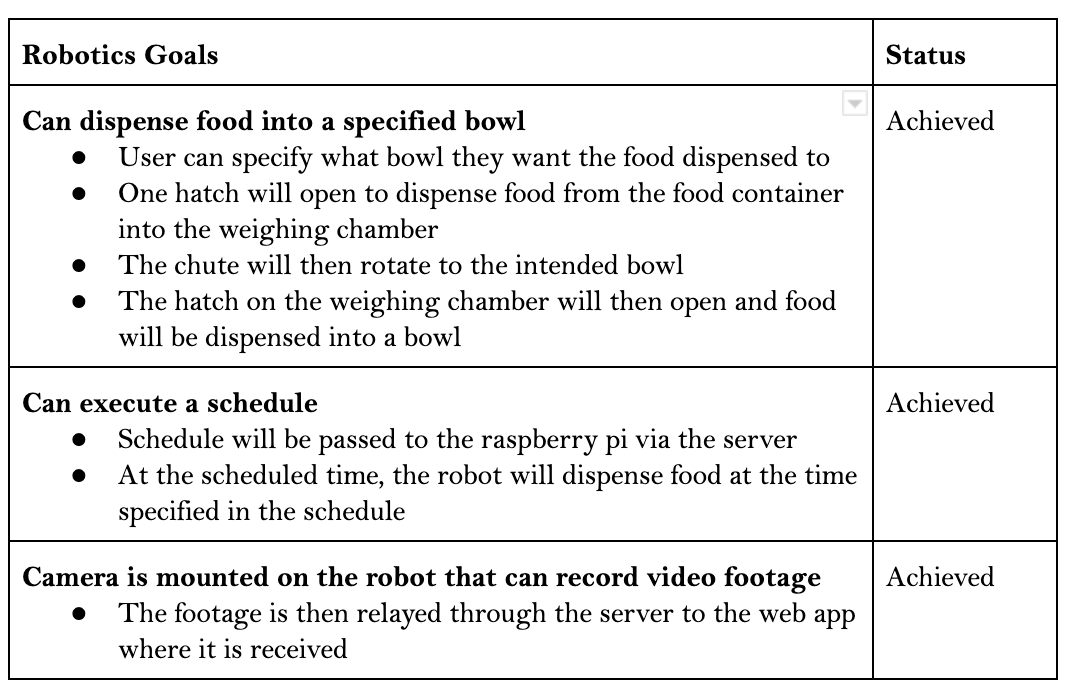
\includegraphics[width=10cm]{robot.png}
 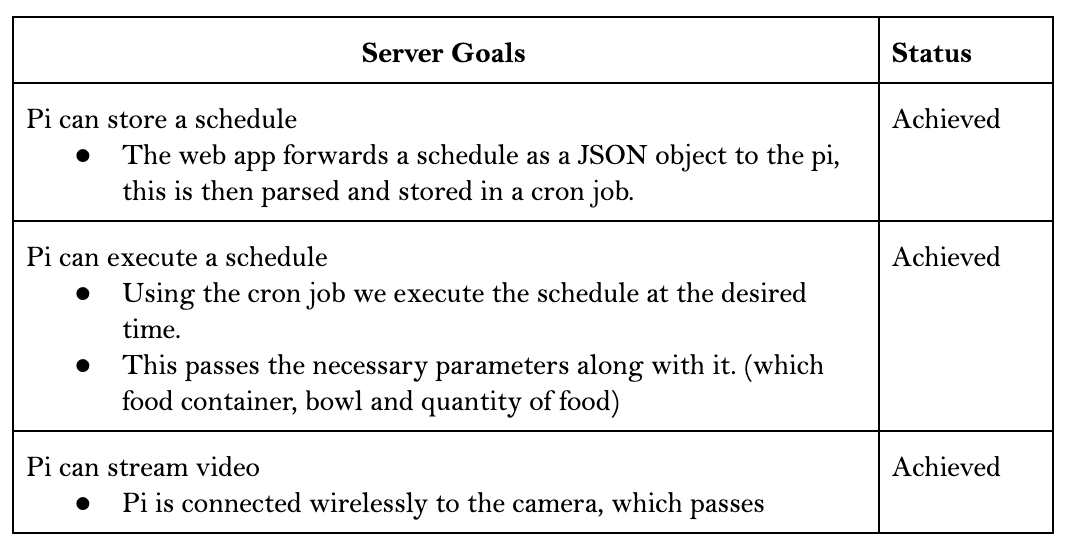
\includegraphics[width=10cm]{server.png}
 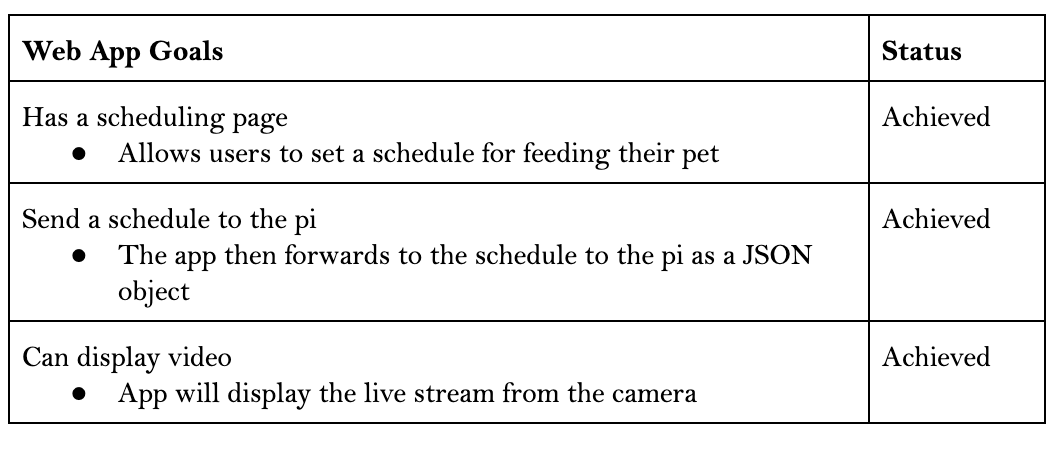
\includegraphics[width=10cm]{app.png}
  }
  \\
  \hline
\end{tabular}
\vskip 5mm


% ------------ORGANISATION----------

\begin{tabular}{|p{\colWidth}|}
	\hline
	\cellcolor{blue!25}\large
	\textbf{Summarise how your group organised the workload to achieve your goals.}
	\\ \hline
	\vtop to 70mm{
We used a sprint setup to maximise our efficiency carrying out tasks. By breaking down our milestones into smaller independent tasks we were able to isolate the specific tasks we needed to do. These would then be worked on by the members of the sub team that the task belonged to. Once we had completed the task, we would archive the card on Trello, giving us a visual representation of how close we were to achieving our milestones. We also had regular meetings to follow up with how tasks were completed and if any changes were necessary. 
To try and make communication easier we did a lot of work together at the same time, whilst this occasionally slightly slower than doing it independently, it meant we were able to communicate much smoother to resolve any issues. This meant that there was a some overlap in what we all worked on. However, the tasks were done primarily as follows:
\begin{itemize}
\item Robotics Hardware - Jerry \& Brodie
\item Robotics Software - Ishan \& Luc
\item Web App - Cuijing \& Asmita
\item Server - Nyal
\end{itemize}
  }
  \\
  \hline
\end{tabular}
\vskip 5mm

% ------------ACHIEVEMENTS----------

\begin{tabular}{|p{\colWidth}|}
	\hline
	\cellcolor{blue!25}\large
	\textbf{What were your main achievements?}
	\\ \hline
	\vtop to 60mm{
Our main achievements were as follows:
\begin{itemize}
\item Live streaming on the camera that is displayed on the web app
\item Sending a schedule from the web app that will then be executed on the pi
\item Executing a schedule that will dispense food at a specified date and time
\item Constructing a modular and extensible robot that can dispense food into two bowls
\end{itemize}
  }
  \\
  \hline
\end{tabular}
\vskip 5mm

% ------------NOT ACHIEVED----------

\begin{tabular}{|p{\colWidth}|}
	\hline
	\cellcolor{blue!25}\large
	\textbf{What did you not achieve? Briefly explain why.}
	\\ \hline
	\vtop to 40mm{
As we decided to prioritise developing features that would make our robot stand out from other competitors in the market, such as live streaming. Thus allowing our robot to become more autonomous and interact more with the world. As a result of this, we were not fully implement the weight sensing feature in our robot. However, we will have this done by the next demo.

  }
  \\
  \hline
\end{tabular}
\vskip 5mm

% ------------QUANTITIVE----------

\begin{tabular}{|p{\colWidth}|}
	\hline
	\cellcolor{blue!25}\large
	\textbf{Include any quantitative data you have collected (this can be a graph/table with a few words)}
	\\ \hline
	\vtop to 200mm{
Analysis for the robot (20 times): This to see the success of the weighing chamber dropping food on to the slide, below are the results:
\begin{itemize}
    \item Complete Success (CS) - all food the in chamber was dispensed with no problems
    \item Partial Success (PS) - the majority of the food in the chamber (over $60\%$) was dispensed with no problems
    \item Partial Failure (PF) -  A significant proportion of food in the chamber was not dispensed (over $60\%$)
    \item Complete Failure (CF) - There was a significant issue with the robot (a part broke or the motor did not run)
    \end{itemize}
    

\begin{center}
\begin{tabular}{||C| C| C| C||}
\hline \hline
 CS & PS & PF & CF \\ \hline
50\% & 30\%  & 20\%  & 0\%   \\
\hline \hline
                    
\end{tabular}
    
\end{center}
  }
  \\
  \hline
\end{tabular}
\vskip 5mm


\begin{tabular}{|p{\colWidth}|}
	\hline
	\cellcolor{blue!25}\large
	\textbf{Include any quantitative data you have collected (this can be a graph/table with a few words)}
	\\ \hline
	\vtop to 200mm{
	\vspace{1mm}
	So overall we gave 10 people to use the app, we first let them go through the app and explore and then ask them to do a series of tasks, this included :
	\begin{itemize}
	    \item Registering as a user
	    \item Making 2 pet profiles 
	    \item Going back to the homepage
	    \item Creating a schedule for one pet 
	    \item Logging out 
	\end{itemize}
	\begin{center}
 \begin{tabular}{||c | c{3cm} | c{3cm} | c{3cm} | c{3cm}||} 
 \hline
  & Registering a user & Create pet profiles& Create a Schedule & Logging out \\ [0.5ex] 
 \hline\hline
 1 & Success  & Success& Success & Success  \\ 
 \hline
 2 & Success  & Success& Success & Success \\
 \hline
 3 & Success  & Success& Success & Success\\
 \hline
 4 & Success  & Success& Success & Success \\
 \hline
  5 & Success  & Success& Success & Success \\
  \hline
   6 & Success  & Success& Success & Success \\
  \hline
   7 & Success  & Success& Success & Success \\
  \hline
   8 & Success  & Success& Success & Success \\
  \hline
   9 & Success  & Success& Success & Success \\
  \hline
 10 & Success  & Success& Success & Success \\ [1ex] 
 \hline
\end{tabular}
\end{center}

  }
  \\
  \hline
\end{tabular}
\vskip 5mm

\begin{tabular}{|p{\colWidth}|}
	\hline
	\cellcolor{blue!25}\large
	\textbf{Include any quantitative data you have collected (this can be a graph/table with a few words)}
	\\ \hline
	\vtop to 200mm{
	While exploring the app, we noticed the app crashed 30\% of the time, this was due to users trying to make a schedule before a pet profile. Users were 100\% successful however when given the series of tasks to complete. Notes from users included:
	\begin{itemize}
	    \item Best to start with one pet and add more if necessary - what if someone only has one pet ?
	    \item Information overload - a lot of info is being seen when you open the app
	    \item Good if some of the text fields were dropdowns selections
	    \item Good to add an image on pet profiles - allows better differentiation
	\end{itemize}

	\vspace{2mm}
	


  }
  \\
  \hline
\end{tabular}
\vskip 5mm

% ------------NEXT STEPS----------

\begin{tabular}{|p{\colWidth}|}
	\hline
	\cellcolor{blue!25}\large
	\textbf{Say briefly what changes you will make to your plan for the next demo.}
	\\ \hline
	\vtop to 45mm{
As we were unable to fully finalize the weight sensing in the robot, we will aim to finalize that before our  next demo. Furthermore, as we have implemented live streaming ahead of schedule, we will consider what other additional features we will add to the robot for the next demo.
In terms of our operations, we need to ensure better quality checking so that we are confident that when we have finished a part of the system, we can be sure that it will function as intended. 

  \\
  \hline
\end{tabular}

\end{center}
  
\end{document}